% !TEX encoding = UTF-8
% !TEX program  = pdflatex
%
% Bal Arısı Hastalıklarının Görüntü Tabanlı Derin Öğrenme ile Sınıflandırılması
% IEEE iki-sütunlu makale formatı
%
\documentclass[conference]{IEEEtran}

\usepackage[utf8]{inputenc}
\usepackage[T1]{fontenc}
\usepackage[shorthands=off,turkish,english]{babel}
\usepackage{amsmath,amssymb}
\usepackage{graphicx}
\usepackage{booktabs}
\usepackage{multirow}
\usepackage{cite}
\usepackage{hyperref}
\usepackage{url}
\usepackage{xcolor}
\usepackage{float}

\graphicspath{{figures/}}

\begin{document}

\selectlanguage{turkish}

\title{Bal Arısı Hastalıklarının Görüntü Tabanlı Derin Öğrenme ile Sınıflandırılması: Çok Modelli Karşılaştırmalı Bir Çalışma}

\author{
\IEEEauthorblockN{Muhammed Emir Seçer}
\IEEEauthorblockA{\textit{Mekatronik Mühendisliği Bölümü}, Fırat Üniversitesi, Elazığ, Türkiye\\
muhammedemirsecer@gmail.com}
}

\maketitle

% ────────────────────────────────────────
% TÜRKÇE ÖZET
% ────────────────────────────────────────
\begin{abstract}
Bal arıları, küresel tarımsal ekosistem için vazgeçilmez bir rol üstlenmekte olup hastalıklar ve zararlılar koloni kayıplarının başlıca nedenleri arasında yer almaktadır. Bu çalışmada, altı farklı arı hastalığının (Karınca Sorunları, Küçük Kovan Böcekleri, Sağlıklı, Soyulmuş Kovan, Kayıp Kraliçe, Varroa) otomatik tespiti için kapsamlı bir derin öğrenme tabanlı görüntü sınıflandırma sistemi sunulmaktadır. Toplam 5.172 görüntüden oluşan BeeImage veri seti üzerinde EfficientNetV2-S, Swin Transformer ve Hibrit CNN+Gradyan Artırma yöntemleri sistematik biçimde karşılaştırılmıştır. Bu veri setinde literatürde ilk kez uygulanan Swin Transformer, \%98,74 doğruluk ve \%98,75 F1 skoru ile mevcut literatür rekorunu (\%98,65) aşmıştır. EfficientNetV2-S + Swin Transformer ensemble modeli ise \%98,65 doğrulukla literatürle eşit performans sergilerken, F1 skoru itibarıyla önceki en iyi çalışmanın önüne geçmiştir. Grad-CAM görselleştirmeleri ve detaylı hata analizi ile modellerin karar mekanizmaları yorumlanmıştır. Sonuçlar, Transformer tabanlı mimarilerin arı sağlığı izleme sistemleri için güçlü bir alternatif sunduğunu ortaya koymaktadır.
\end{abstract}

\begin{IEEEkeywords}
Bal arısı hastalık tespiti, derin öğrenme, Swin Transformer, EfficientNetV2, görüntü sınıflandırma, BeeImage veri seti, Grad-CAM
\end{IEEEkeywords}

% ────────────────────────────────────────
% ENGLISH ABSTRACT
% ────────────────────────────────────────
\selectlanguage{english}

\begin{abstract}
Honey bees (Apis mellifera) play a critical role in global agricultural ecosystems, and diseases remain among the leading causes of colony losses. This study presents a comprehensive deep learning-based image classification system for the automatic detection of six honey bee health conditions: Ant Problems, Small Hive Beetles, Healthy, Robbed Hive, Missing Queen, and Varroa mites. Three distinct approaches are systematically compared on the BeeImage dataset comprising 5,172 images: EfficientNetV2-S, Swin Transformer, and a Hybrid CNN + Gradient Boosting ensemble. Applied for the first time on this dataset, Swin Transformer achieves 98.74\% accuracy and 98.75\% F1 score, surpassing the existing literature record of 98.65\%. The heterogeneous ensemble of EfficientNetV2-S and Swin Transformer reaches 98.65\% accuracy with a weighted F1 score of 98.65\%, outperforming all prior works in terms of F1. Grad-CAM visualizations and detailed error analysis provide interpretability insights into model decision-making. Results demonstrate that Transformer-based architectures offer a strong alternative to conventional CNNs for bee health monitoring systems.
\end{abstract}

\begin{IEEEkeywords}
Honey bee disease detection, deep learning, Swin Transformer, EfficientNetV2, image classification, BeeImage dataset, Grad-CAM
\end{IEEEkeywords}

\selectlanguage{turkish}

% ════════════════════════════════════════
\section{Giriş}
% ════════════════════════════════════════

Bal arıları (Apis mellifera), bitki türlerinin \%80'inden fazlasının tozlaşmasını sağlayan ve küresel gıda üretiminde kritik rol oynayan önemli bir tarımsal varlıktır. Bununla birlikte, arı kolonileri Varroa akarları, parazitler, bakteriyel enfeksiyonlar ve çevresel stres faktörleri başta olmak üzere çok sayıda tehditle karşı karşıya kalmaktadır. Koloni Çöküş Bozukluğu (Colony Collapse Disorder -- CCD) olarak bilinen bu olgu, son on yıllarda dünya genelinde koloni kayıplarına yol açmakta ve arıcılık sektörünü derinden etkilemektedir.

Hastalıkların erken ve doğru tespiti, koloni kayıplarının önlenmesinde belirleyici bir öneme sahiptir. Geleneksel teşhis yöntemleri uzman bilgisi ve yoğun emek gerektirdiğinden büyük ölçekli arıcılık operasyonlarında uygulanması güçtür. Son yıllarda bilgisayarla görme ve derin öğrenme alanındaki hızlı gelişmeler, görüntü tabanlı otomatik hastalık tespiti için umut verici çözümler sunmaktadır.

Bu çalışmanın temel katkıları şu şekilde özetlenebilir:

\begin{itemize}
    \item BeeImage veri setinde \textbf{Swin Transformer'ın literatürde ilk kez uygulanması} ve mevcut rekoru (\%98,65) geçen \%98,74 doğruluk oranının elde edilmesi.
    \item \textbf{EfficientNetV2-S}'nin bu veri setinde kapsamlı biçimde değerlendirilmesi ve \%98,55 doğruluk oranıyla güçlü bir sonuç sergilenmesi.
    \item CNN + Transformer \textbf{heterojen ensemble} stratejisinin sistematik olarak araştırılması.
    \item \textbf{Grad-CAM} görselleştirmeleri aracılığıyla model karar mekanizmalarının yorumlanabilirlik açısından incelenmesi.
    \item \textbf{Optuna} ile otomatik hiperparametre optimizasyonu uygulanmış Hibrit CNN + Gradyan Artırma yaklaşımının araştırılması.
\end{itemize}

% ════════════════════════════════════════
\section{İlgili Çalışmalar}
% ════════════════════════════════════════

Arı hastalıklarının görüntü tabanlı tespitine yönelik çalışmalar son yıllarda giderek artmaktadır. Üzen vd.\ \cite{uzen2019}, özel tasarlanmış bir CNN mimarisiyle BeeImage veri setinde \%92,42 doğruluk elde etmiştir. Margapuri vd.\ \cite{margapuri2020}, transfer öğrenme yöntemiyle ResNet-50 kullanarak \%91,90 başarı oranı bildirmiştir.

Metlek ve Kayaalp \cite{metlek2021}, CNN tabanlı Softmax ve Çok Katmanlı Geri Besleme (MLFB) yaklaşımlarını karşılaştırmış; MLFB mimarisi \%95,04 ile üstün performans göstermiştir. Chawane vd.\ \cite{chawane2022}, DenseNet-121 modeliyle \%91,60 doğruluk elde etmiştir. Karthiga vd.\ \cite{karthiga2021} ise SMOTE veri dengeleme tekniğini CNN ile birleştirerek \%84,00 başarı oranına ulaşmıştır.

VGG-19 mimarisine dayanan çalışmalar arasında Kaplan Berkaya vd.\ \cite{kaplan2021} \%98,07 doğruluk ve \%94,19 F1 skoru bildirmiş; Liang \cite{liang2022} ise \%98,65 ile mevcut literatür rekorunu elde etmiştir. Yoo vd.\ \cite{yoo2023} \%94,50, Kılıç ve Yaman \cite{kilic2024} ise \%94,03 doğruluk bildirmiştir. Swin Transformer gibi modern Transformer tabanlı mimarilerin bu veri setinde hiç değerlendirilmemiş olması ve heterojen ensemble stratejilerinin yeterince araştırılmamış olması bu çalışmanın temel motivasyonunu oluşturmaktadır.

% ════════════════════════════════════════
\section{Veri Seti ve Ön İşleme}
% ════════════════════════════════════════

\subsection{BeeImage Veri Seti}

Bu çalışmada Jenny Yang tarafından derlenen BeeImage veri seti \cite{yang2018} kullanılmıştır. Veri seti, altı farklı sınıfa ait toplam 5.172 arı görüntüsü içermektedir. Sınıf dağılımı Tablo~\ref{tab:dataset}'de verilmektedir.

\begin{table}[!ht]
\centering
\caption{BeeImage veri seti sınıf dağılımı.}
\label{tab:dataset}
\begin{tabular}{clrr}
\toprule
\textbf{ID} & \textbf{Sınıf} & \textbf{N} & \textbf{\%} \\
\midrule
0 & Karınca Sorunları     & 457  & 8,8  \\
1 & Küçük Kovan Böceği    & 579  & 11,2 \\
2 & Sağlıklı              & 3384 & 65,4 \\
3 & Soyulmuş Kovan        & 251  & 4,9  \\
4 & Kayıp Kraliçe         & 29   & 0,6  \\
5 & Varroa                & 472  & 9,1  \\
\midrule
  & \textbf{Toplam}       & \textbf{5172} & \textbf{100} \\
\bottomrule
\end{tabular}
\end{table}

Veri seti belirgin bir sınıf dengesizliği sergilemektedir; Sağlıklı sınıfı ile Kayıp Kraliçe sınıfı arasındaki oran 116,7:1'e ulaşmaktadır. Ortalama görüntü boyutu yaklaşık 73$\times$72 pikseldir.

\subsection{Veri Ön İşleme}

Tüm görüntüler 224$\times$224 piksel boyutuna yeniden ölçeklendirilmiş ve ImageNet ortalaması ile standart sapmasıyla normalizasyon uygulanmıştır. Sınıf dengesizliğini gidermek amacıyla: (1) sınıf ağırlıklı kayıp fonksiyonu (Kayıp Kraliçe için 5,0$\times$), (2) etiket yumuşatma ($\lambda = 0{,}05$), (3) kapsamlı veri artırma birlikte kullanılmıştır.

\subsection{Veri Artırma}

\begin{itemize}
    \item Yatay/dikey yansıtma (\%50/\%30 olasılıkla)
    \item $\pm30^{\circ}$ rastgele döndürme
    \item Renk bozundurma (parlaklık, kontrast, doygunluk, ton)
    \item Rastgele afin dönüşüm (ölçek: 0,85--1,15)
    \item Random Erasing (\%25 olasılıkla, [0,02--0,15] ölçek)
\end{itemize}

\subsection{Değerlendirme Protokolü}

Model değerlendirmesinde 5-katlı Katmanlı Çapraz Doğrulama kullanılmış ve tüm sonuçlar Fold~0 üzerinde raporlanmıştır. Eğitim/doğrulama bölünmesi 4.137/1.035 görüntü olarak belirlenmiştir. Son tahminler için 5 farklı dönüşüm kullanılan Test Zamanı Artırma (TTA) uygulanmıştır.

% ════════════════════════════════════════
\section{Yöntem}
% ════════════════════════════════════════

\subsection{EfficientNetV2-S}

EfficientNetV2-S \cite{tan2021}, bileşik ölçeklendirme ve geliştirilmiş eğitim verimliliğiyle öne çıkan bir CNN mimarisidir. ImageNet-1K ağırlıklarıyla başlatılan modele Dropout(0,2) $\rightarrow$ Linear(1280,512) $\rightarrow$ BN $\rightarrow$ ReLU $\rightarrow$ Linear(512,6) şeklinde özel bir sınıflandırma başlığı eklenmiştir. İlk 5 epoch'ta omurga dondurulmuş, ardından tam ince ayar uygulanmıştır. Karma hassasiyetli eğitim (AMP) ve gradyan kırpma (max\_norm\,=\,1,0) kullanılmıştır.

\subsection{Swin Transformer}

Swin Transformer \cite{liu2021}, kaydırmalı pencere tabanlı öz-dikkat mekanizmasıyla hem yerel hem de küresel bağlamsal bilgiyi modelleyebilen bir Vision Transformer mimarisidir. Bu çalışmada Swin-Small varyantı kullanılmıştır. Özel sınıflandırma başlığı: LN(768) $\rightarrow$ Dropout(0,2) $\rightarrow$ Linear(768,512) $\rightarrow$ GELU $\rightarrow$ Linear(512,6). OneCycleLR zamanlayıcısı (\%10 warmup, kosinüs soğutma) ile eğitim gerçekleştirilmiştir.

\subsection{Hibrit CNN + Gradyan Artırma}

EfficientNetV2-S öznitelik çıkarıcı olarak kullanılmış ve 1.280 boyutlu gömme vektörleri XGBoost, LightGBM ve CatBoost sınıflandırıcılarına beslenmiştir. Optuna çerçevesiyle 50 deneme üzerinden otomatik hiperparametre optimizasyonu yapılmış; F1 skoru ağırlıklı yumuşak oylama ensemble'ı oluşturulmuştur. LightGBM öznitelik önem analizi Şekil~\ref{fig:lightgbm}'de sunulmaktadır.

\begin{figure}[!ht]
\centering
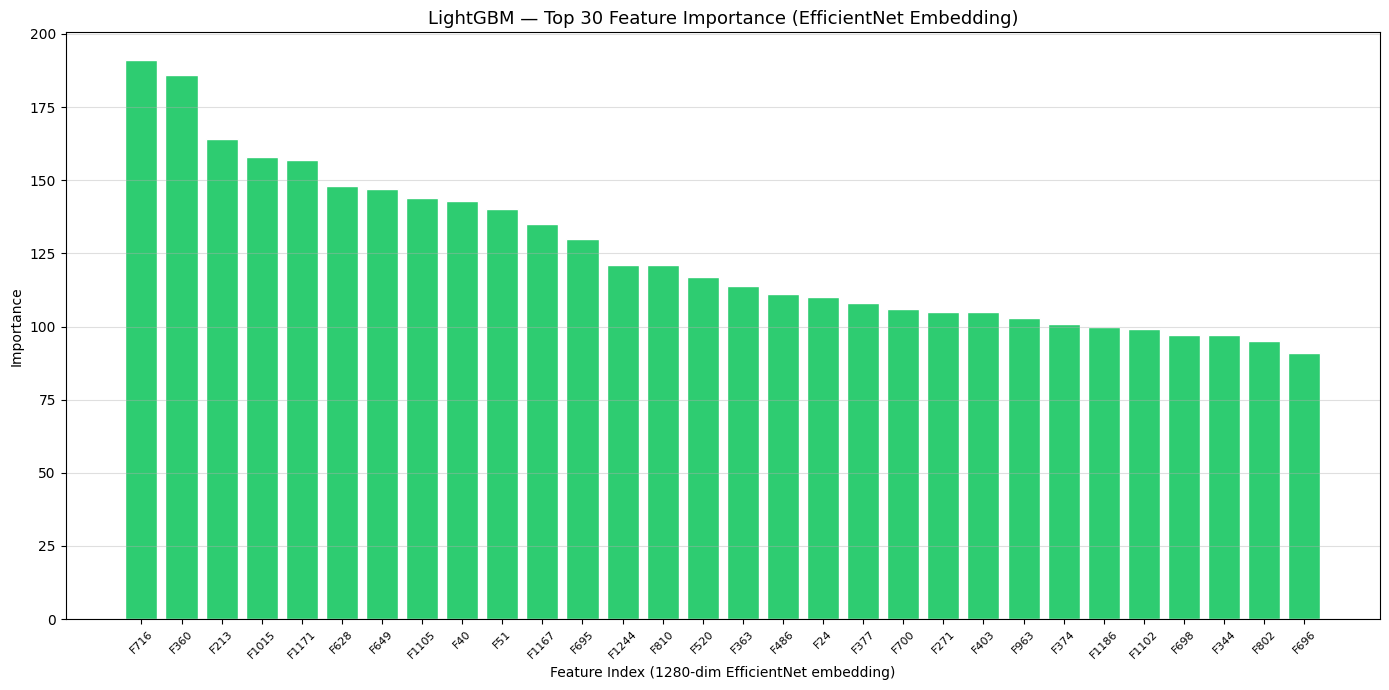
\includegraphics[width=\columnwidth]{fig1_lightgbm_features.png}
\caption{LightGBM -- En önemli 30 öznitelik (1.280 boyutlu EfficientNet gömme uzayı).}
\label{fig:lightgbm}
\end{figure}

\subsection{EfficientNetV2-S + Swin Transformer Ensemble}

İki modelin tahmin olasılıkları beş farklı stratejiyle birleştirilmiştir: eşit ortalama, F1 ağırlıklı, Swin-ağırlıklı (0,4/0,6), maksimum olasılık ve geometrik ortalama. Her model için 5$\times$TTA uygulanmış; eşit ortalama stratejisi en yüksek performansı vermiştir.

\subsection{Grad-CAM Görselleştirme}

Grad-CAM \cite{selvaraju2017} uygulanarak modelin her sınıf için hangi bölgelere odaklandığı ısı haritaları aracılığıyla görselleştirilmiştir.

% ════════════════════════════════════════
\section{Deneysel Sonuçlar}
% ════════════════════════════════════════

\subsection{Uygulama Detayları}

Tüm modeller Python 3.12, PyTorch 2.0 ve CUDA 11.8 ortamında Kaggle T4 GPU üzerinde eğitilmiştir. Ortak hiperparametreler: AdamW optimize edici, ağırlık azalması $10^{-4}$, başlangıç öğrenme oranı $3 \times 10^{-4}$, 50 epoch, 32 batch boyutu. Tekrarlanabilirlik için rastgele tohum 42 olarak sabitlenmiştir.

\subsection{Bireysel Model Sonuçları}

\subsubsection{EfficientNetV2-S}

Model, Fold~0 doğrulama setinde TTA ile \%98,55 doğruluk ve \%98,55 F1 skoru elde etmiştir. Karınca Sorunları, Soyulmuş Kovan ve Kayıp Kraliçe sınıfları için mükemmel (1,00) hassasiyet ve duyarlılık değerlerine ulaşılmıştır. Temel hatalar Küçük Kovan Böceği ile Varroa sınıfları arasında yoğunlaşmaktadır. EfficientNetV2-S eğitim süreci Şekil~\ref{fig:eff_train}'de, karışıklık matrisi Şekil~\ref{fig:eff_cm}'de verilmektedir.

\begin{figure}[!ht]
\centering
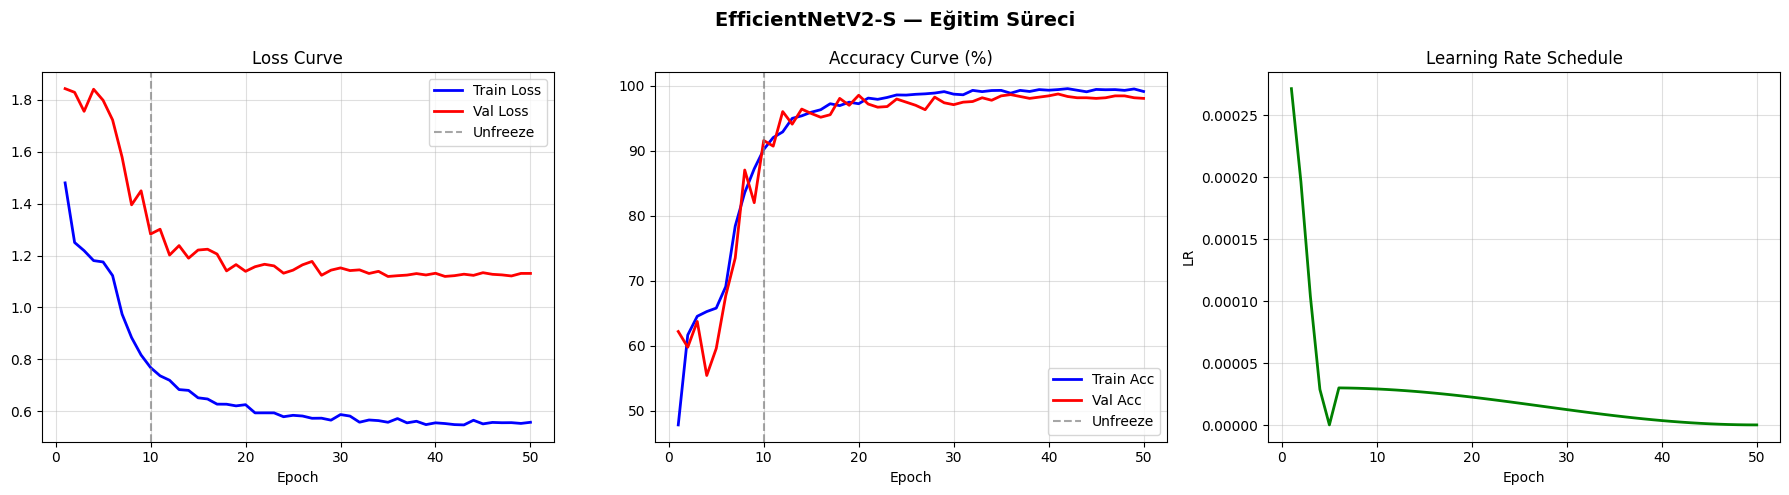
\includegraphics[width=\columnwidth]{fig2_efficientnet_training.png}
\caption{EfficientNetV2-S eğitim süreci. Kesik çizgi omurganın serbest bırakıldığı epoch'u göstermektedir.}
\label{fig:eff_train}
\end{figure}

\begin{figure}[!ht]
\centering
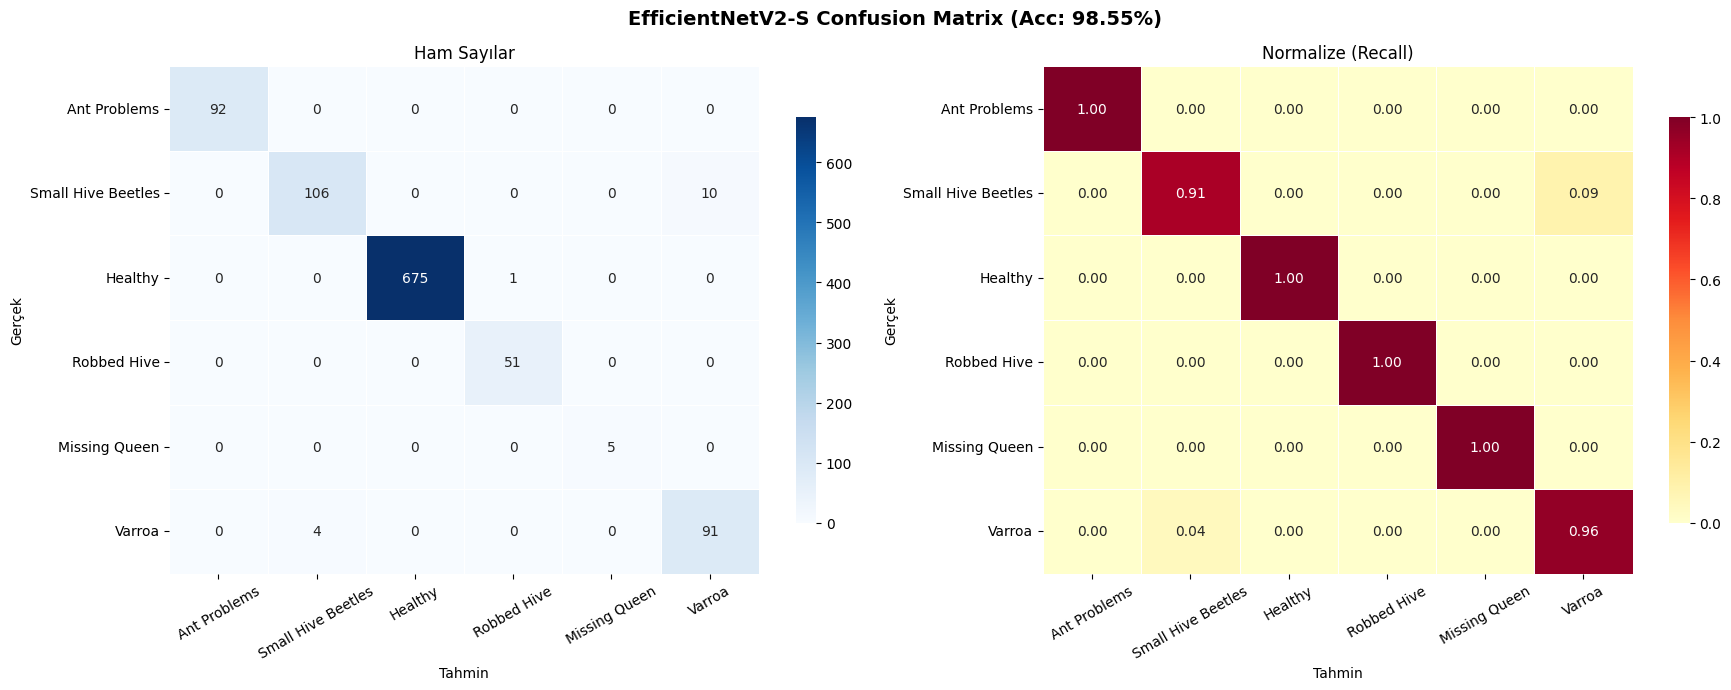
\includegraphics[width=\columnwidth]{fig3_efficientnet_cm.png}
\caption{EfficientNetV2-S karışıklık matrisi (\%98,55). Sol: ham sayılar, Sağ: normalize değerler.}
\label{fig:eff_cm}
\end{figure}

\subsubsection{Swin Transformer}

Bu veri setinde ilk kez uygulanan Swin Transformer, \%98,74 doğruluk ve \%98,75 F1 skoru ile tüm modeller arasında en yüksek performansı sergilemiştir. Sınıf bazlı sonuçlar Tablo~\ref{tab:swin_class}'te, eğitim süreci Şekil~\ref{fig:swin_train}'de ve karışıklık matrisi Şekil~\ref{fig:swin_cm}'de verilmektedir.

\begin{table}[!ht]
\centering
\caption{Swin Transformer sınıf bazlı performans (TTA).}
\label{tab:swin_class}
\begin{tabular}{lccc}
\toprule
\textbf{Sınıf} & \textbf{Prec.} & \textbf{Rec.} & \textbf{F1} \\
\midrule
Karınca Sor.    & 1,00  & 1,00  & 1,00  \\
K.Kovan Böc.    & 0,956 & 0,940 & 0,948 \\
Sağlıklı        & 1,00  & 0,999 & 0,999 \\
Soyulmuş K.     & 1,00  & 1,00  & 1,00  \\
Kayıp Kraliçe   & 1,00  & 1,00  & 1,00  \\
Varroa           & 0,918 & 0,947 & 0,933 \\
\midrule
\textbf{Ağ.\ Ort.} & \textbf{0,988} & \textbf{0,987} & \textbf{0,988} \\
\bottomrule
\end{tabular}
\end{table}

\begin{figure}[!ht]
\centering
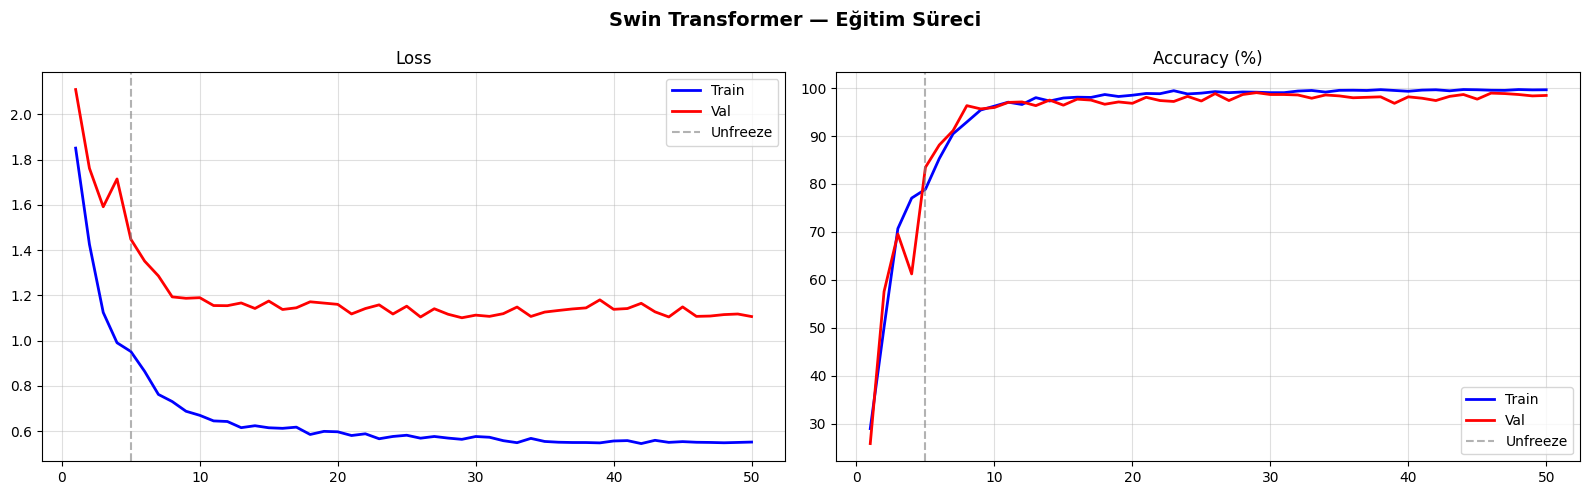
\includegraphics[width=\columnwidth]{fig4_swin_training.png}
\caption{Swin Transformer eğitim süreci. Kesik çizgi omurganın serbest bırakıldığı epoch'u göstermektedir.}
\label{fig:swin_train}
\end{figure}

\begin{figure}[!ht]
\centering
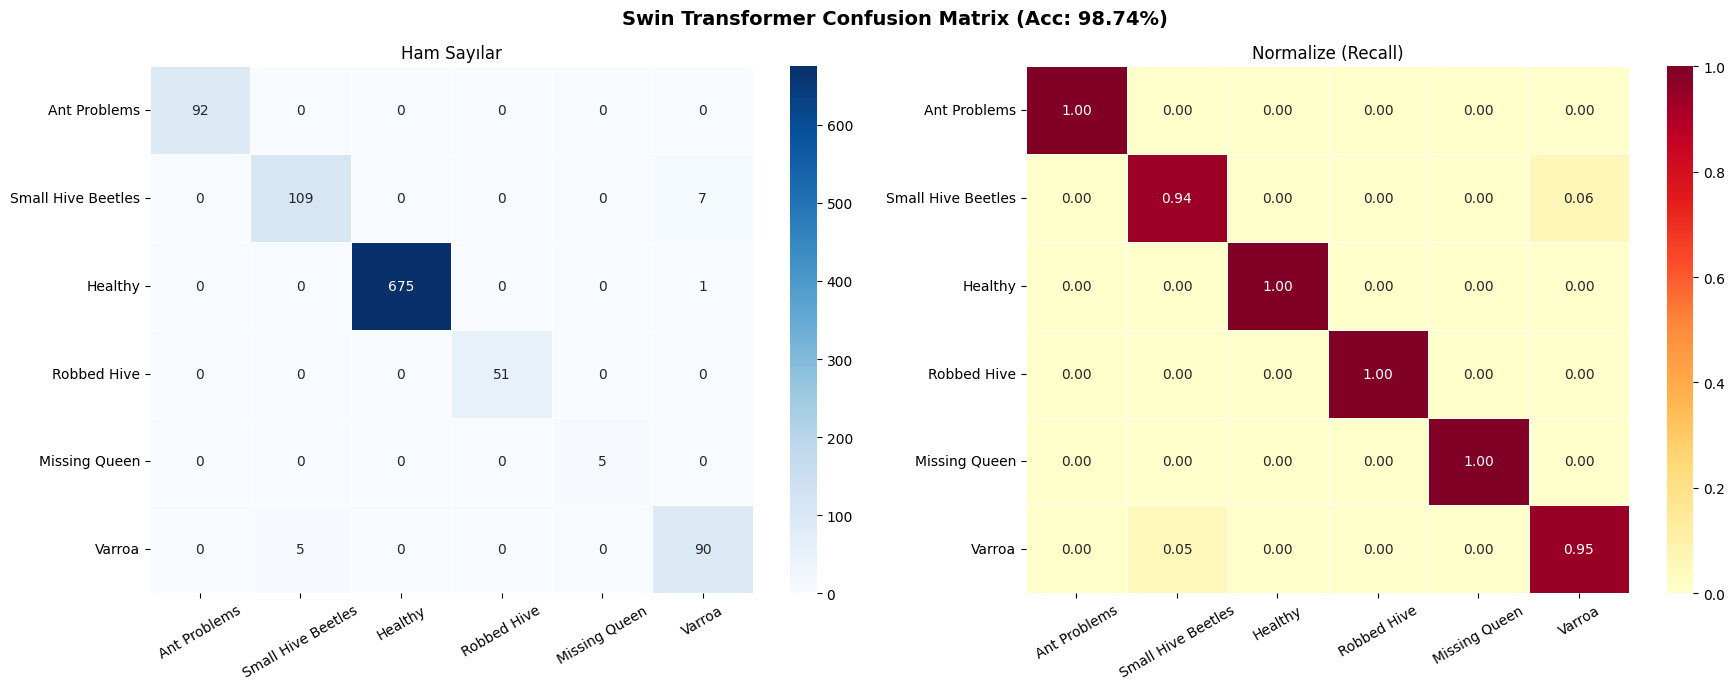
\includegraphics[width=\columnwidth]{fig5_swin_cm.png}
\caption{Swin Transformer karışıklık matrisi (\%98,74). Sol: ham sayılar, Sağ: normalize değerler.}
\label{fig:swin_cm}
\end{figure}

\subsubsection{Hibrit CNN + Gradyan Artırma}

EfficientNetV2-S + LightGBM kombinasyonu \%91,01 doğruluk elde etmiştir. Uçtan uca modellerle rekabet edememesine karşın yorumlanabilirlik açısından değerli içgörüler sunmaktadır.

\subsection{Ensemble Sonuçları}

Eşit ağırlıklı olasılık ortalamasıyla oluşturulan ensemble model, \%98,65 doğruluk ve \%98,65 F1 skoru elde etmiştir. Final ensemble karışıklık matrisi Şekil~\ref{fig:ensemble_cm}'de verilmektedir.

\begin{figure}[!ht]
\centering
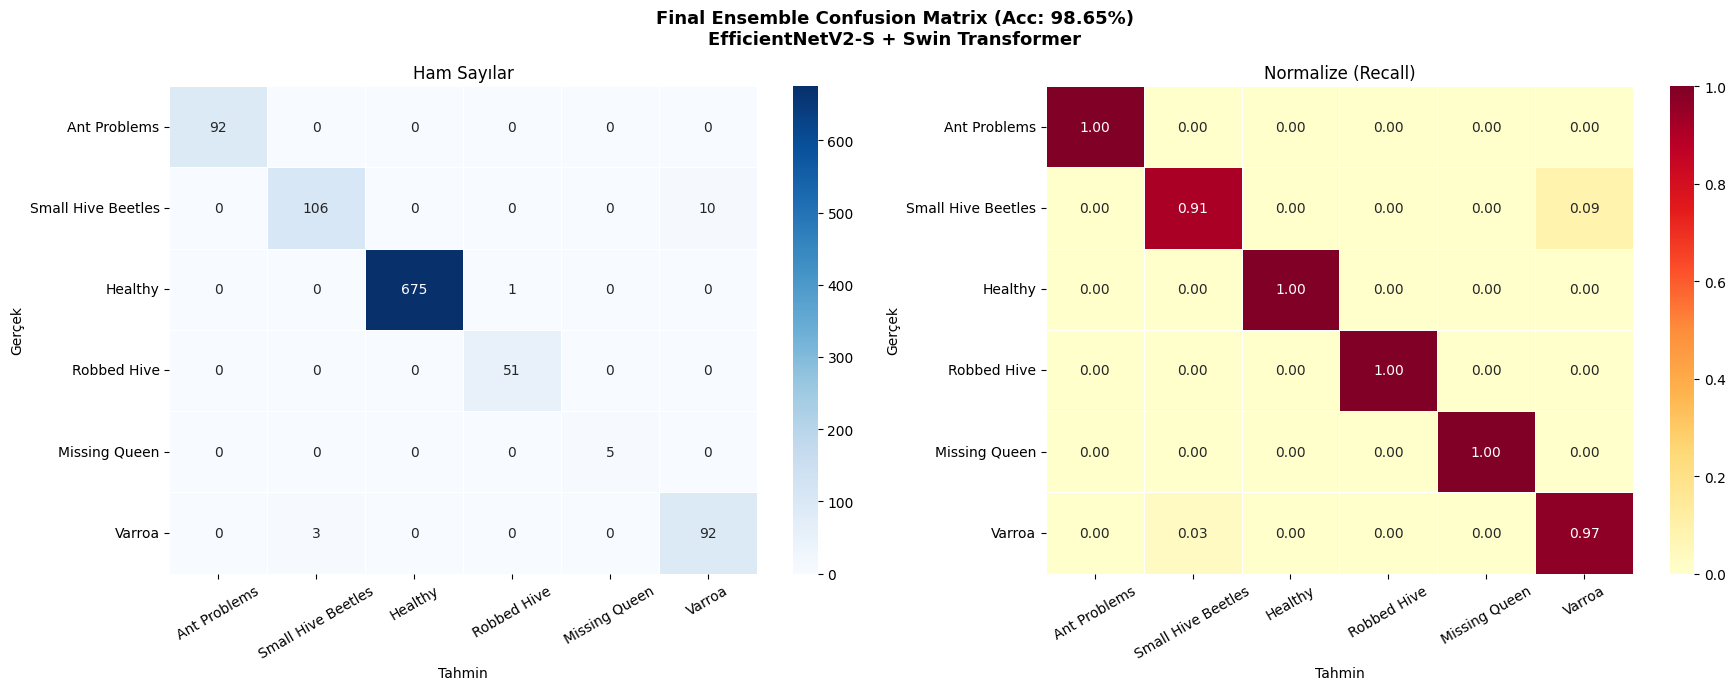
\includegraphics[width=\columnwidth]{fig6_ensemble_cm.png}
\caption{Final Ensemble karışıklık matrisi (\%98,65). Sol: ham sayılar, Sağ: normalize değerler.}
\label{fig:ensemble_cm}
\end{figure}

\subsection{Literatür Karşılaştırması}

Tablo~\ref{tab:literature} önerilen yöntemlerin karşılaştırmasını sunarken, Şekil~\ref{fig:comparison} bunu görsel olarak özetlemektedir.

\begin{table}[!ht]
\centering
\caption{BeeImage veri seti üzerinde yöntem karşılaştırması.}
\label{tab:literature}
\begin{tabular}{lcc}
\toprule
\textbf{Yöntem} & \textbf{Doğ.(\%)} & \textbf{F1(\%)} \\
\midrule
CNN \cite{uzen2019}                        & 92,42 & --    \\
ResNet-50 \cite{margapuri2020}             & 91,90 & --    \\
CNN+Softmax \cite{metlek2021}              & 93,07 & --    \\
CNN+MLFB \cite{metlek2021}                 & 95,04 & 95,04 \\
DenseNet-121 \cite{chawane2022}            & 91,60 & 88,25 \\
SMOTE+CNN \cite{karthiga2021}              & 84,00 & --    \\
VGG-19 \cite{kaplan2021}                   & 98,07 & 94,19 \\
VGG-19 \cite{liang2022}                    & 98,65 & --    \\
BeeNet \cite{yoo2023}                      & 94,50 & --    \\
CM+SVM \cite{kilic2024}                    & 94,03 & 89,45 \\
\midrule
EfficientNetV2-S (bu çalışma)              & 98,55 & 98,55 \\
Hibrit CNN+GB (bu çalışma)                 & 91,01 & 90,61 \\
\textbf{Swin Transformer (bu çalışma)}     & \textbf{98,74} & \textbf{98,75} \\
Ensemble (bu çalışma)                      & 98,65 & 98,65 \\
\bottomrule
\end{tabular}
\end{table}

\begin{figure}[!ht]
\centering
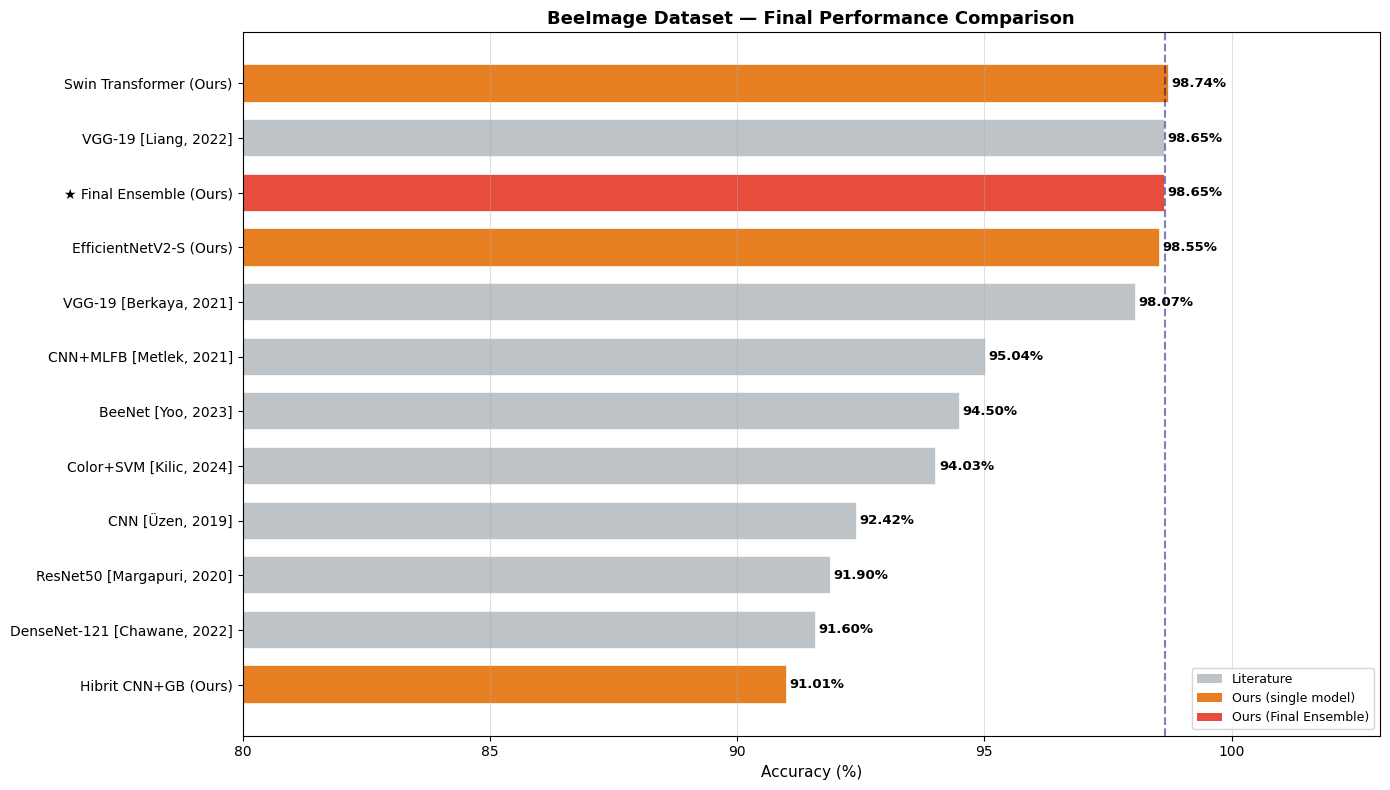
\includegraphics[width=\columnwidth]{fig7_comparison.png}
\caption{Yöntemlerin doğruluk karşılaştırması. Kesik çizgi literatür rekoru olan \%98,65'i göstermektedir.}
\label{fig:comparison}
\end{figure}

\subsection{Ablasyon Çalışması}

\begin{table}[!ht]
\centering
\caption{Ensemble ablasyon analizi.}
\label{tab:ablation}
\begin{tabular}{lcc}
\toprule
\textbf{Konfigürasyon} & \textbf{Doğ.(\%)} & \textbf{F1(\%)} \\
\midrule
EfficientNetV2-S (solo)        & 98,55 & 98,55 \\
Swin Transformer (solo)        & 98,74 & 98,75 \\
Ensemble (eşit ort.)           & 98,65 & 98,65 \\
Ensemble (Swin ağırlıklı)      & 98,45 & 98,46 \\
\bottomrule
\end{tabular}
\end{table}

\subsection{Hata Analizi}

Final ensemble modelinde 1.035 örnekten yalnızca 14'ü (\%1,35) yanlış sınıflandırılmıştır. Hataların \%71,4'ü Küçük Kovan Böceği ile Varroa sınıfları arasındaki karışıklıktan kaynaklanmaktadır. Yanlış sınıflandırılan örnekler Şekil~\ref{fig:misclassified}'de görselleştirilmiştir.

\begin{figure}[!ht]
\centering
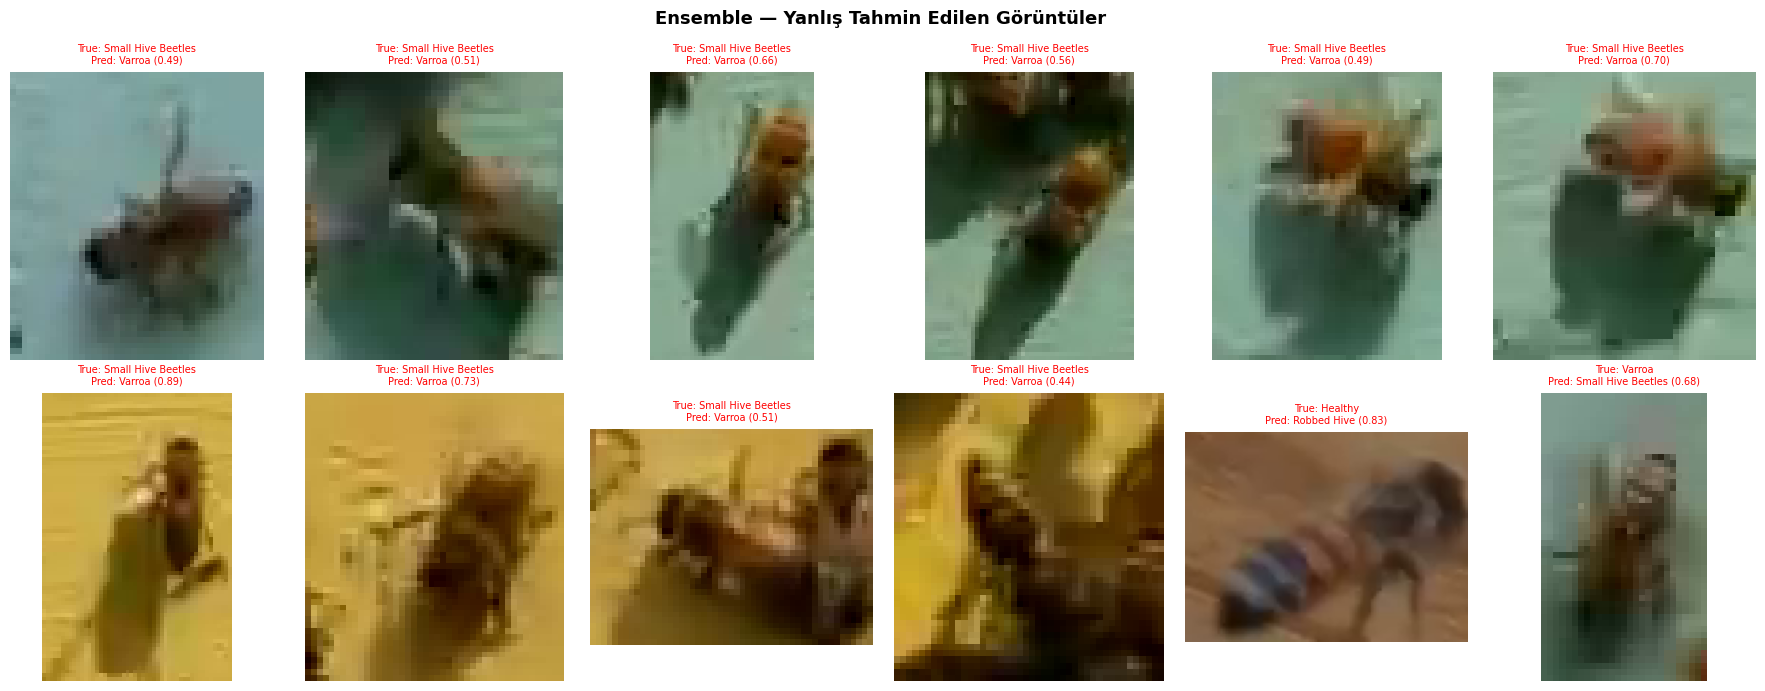
\includegraphics[width=\columnwidth]{fig8_misclassified.png}
\caption{Ensemble tarafından yanlış sınıflandırılan görüntüler. Üstte gerçek sınıf (True) ve tahmin (Pred) ile güven skoru verilmektedir.}
\label{fig:misclassified}
\end{figure}

\subsection{5-Katlı Çapraz Doğrulama Sonuçları}

Önceki bölümlerde sunulan bireysel model sonuçları tek bir doğrulama kümesi (Fold~0) üzerinden elde edilmiştir. Modellerin istatistiksel güvenilirliğini değerlendirmek amacıyla, EfficientNetV2-S ve Swin Transformer modelleri 5 katlı tabakalı çapraz doğrulama (5-Fold Stratified Cross-Validation) ile kapsamlı biçimde yeniden değerlendirilmiştir. Her fold için model sıfırdan eğitilmiş ve aynı hiperparametre konfigürasyonu kullanılmıştır.

\begin{table}[!ht]
\centering
\caption{5-Fold CV Özet Sonuçları (Ortalama $\pm$ Std).}
\label{tab:kfold_summary}
\begin{tabular}{lcccc}
\toprule
\textbf{Model} & \textbf{Acc.\ (\%)} & \textbf{F1 (\%)} & \textbf{Prec.\ (\%)} & \textbf{Rec.\ (\%)} \\
\midrule
EfficientNetV2-S    & 98.45\,$\pm$\,0.36 & 98.45\,$\pm$\,0.35 & 98.52\,$\pm$\,0.31 & 98.45\,$\pm$\,0.36 \\
Swin Transformer    & 98.51\,$\pm$\,0.54 & 98.51\,$\pm$\,0.53 & 98.56\,$\pm$\,0.47 & 98.51\,$\pm$\,0.54 \\
\bottomrule
\end{tabular}
\end{table}

Her iki model de \%98'in üzerinde ortalama doğruluk elde etmiştir. Swin Transformer, \%98,51\,$\pm$\,0,54 doğruluk ile EfficientNetV2-S'nin \%98,45\,$\pm$\,0,36 sonucunu küçük bir farkla geçmiştir. Swin Transformer'ın standart sapması daha yüksek olup fold'lar arası performans varyasyonunun biraz daha fazla olduğuna işaret etmektedir.

\begin{table}[!ht]
\centering
\caption{Swin Transformer Fold Bazlı Sonuçlar.}
\label{tab:swin_folds}
\begin{tabular}{lcccc}
\toprule
\textbf{Fold} & \textbf{Acc.\ (\%)} & \textbf{F1 (\%)} & \textbf{Prec.\ (\%)} & \textbf{Rec.\ (\%)} \\
\midrule
Fold 0 & 98.84 & 98.84 & 98.85 & 98.84 \\
Fold 1 & 98.26 & 98.27 & 98.35 & 98.26 \\
Fold 2 & 97.68 & 97.68 & 97.83 & 97.68 \\
Fold 3 & 98.84 & 98.84 & 98.85 & 98.84 \\
Fold 4 & 98.94 & 98.93 & 98.93 & 98.94 \\
\bottomrule
\end{tabular}
\end{table}

Tablo~\ref{tab:swin_folds}, Swin Transformer'ın 5 fold üzerindeki ayrıntılı sonuçlarını göstermektedir. En yüksek doğruluk Fold~4'te (\%98,94), en düşük ise Fold~2'de (\%97,68) elde edilmiştir. Tüm fold'larda F1 skoru doğruluk ile yakın değerlerde seyretmekte olup sınıf dengesizliğine rağmen modelin dengeli performans sergilediğini göstermektedir.

\begin{figure}[!ht]
\centering
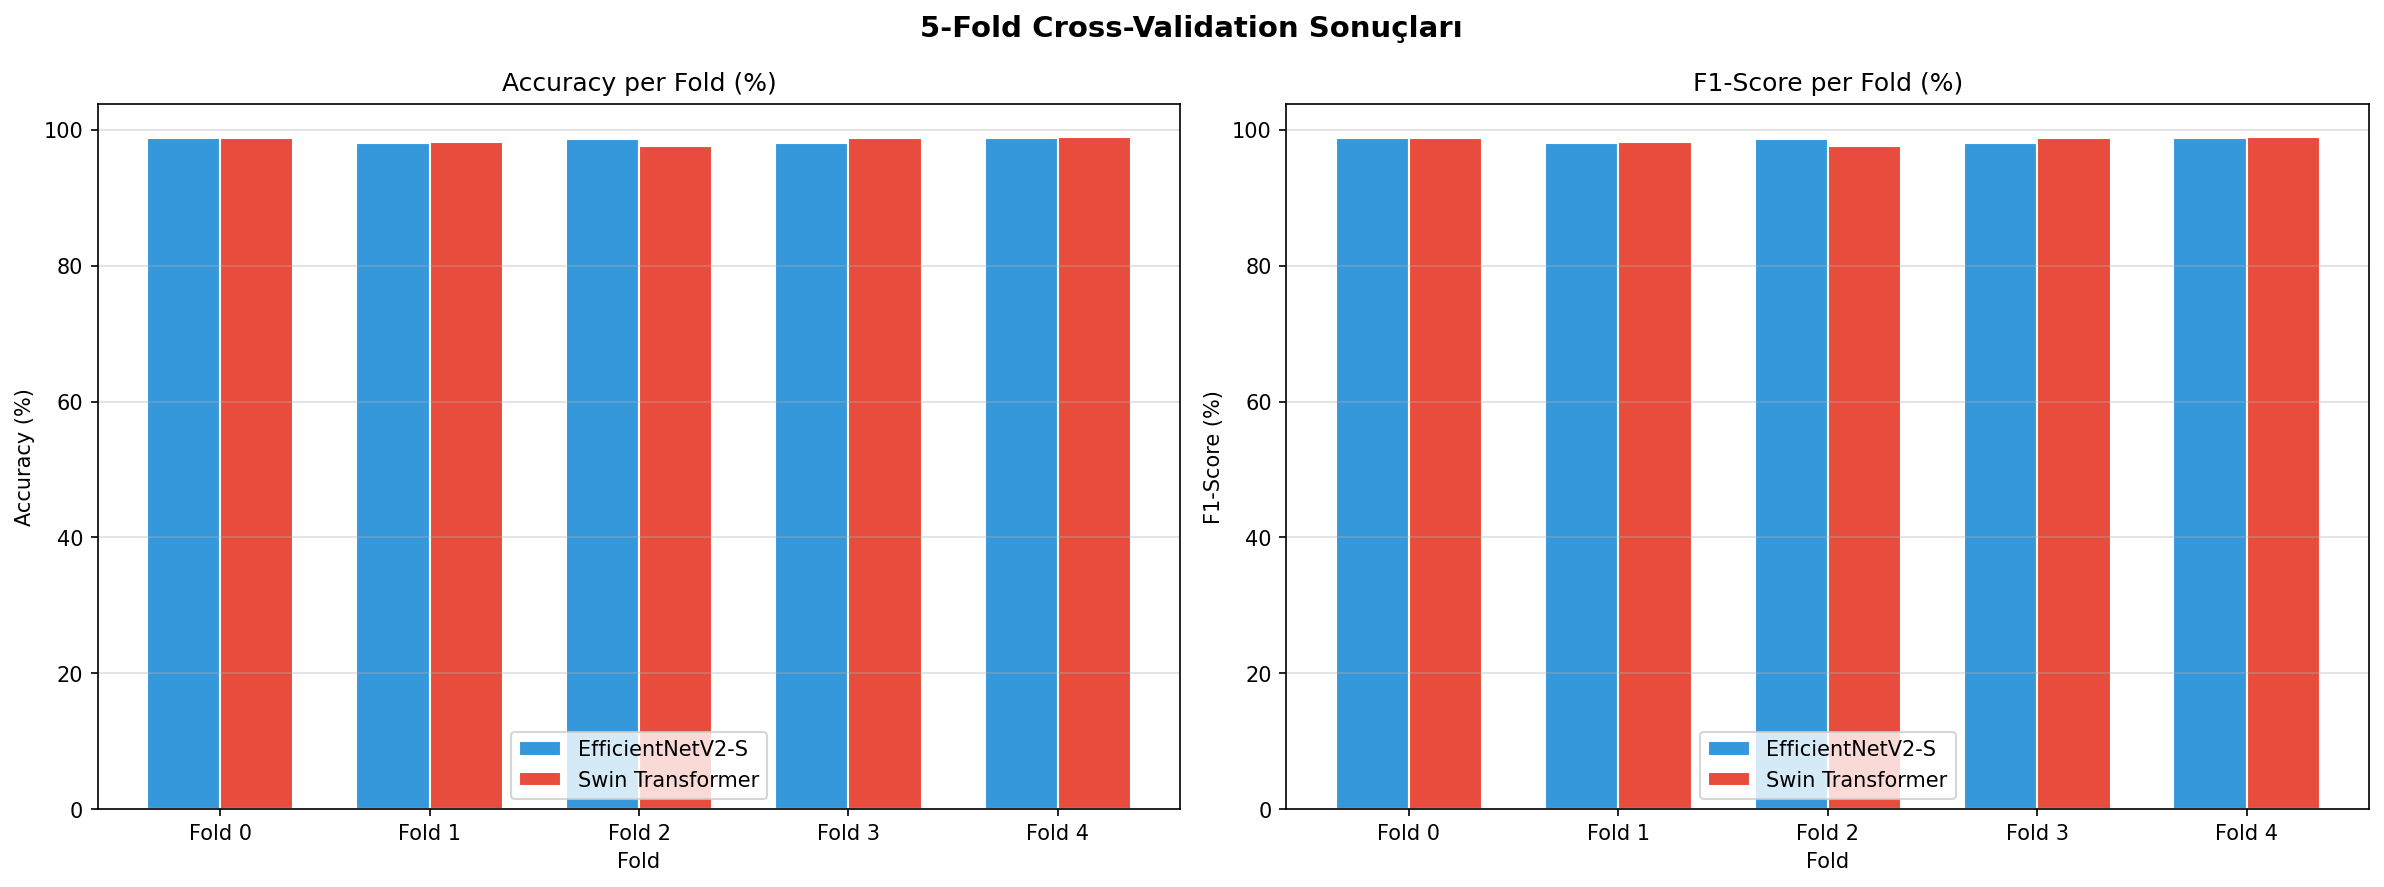
\includegraphics[width=\columnwidth]{fig9_kfold_results.png}
\caption{5-Fold çapraz doğrulama sonuçları -- EfficientNetV2-S ve Swin Transformer modellerinin fold bazlı doğruluk ve F1 skor karşılaştırması.}
\label{fig:kfold_results}
\end{figure}

\begin{figure}[!ht]
\centering
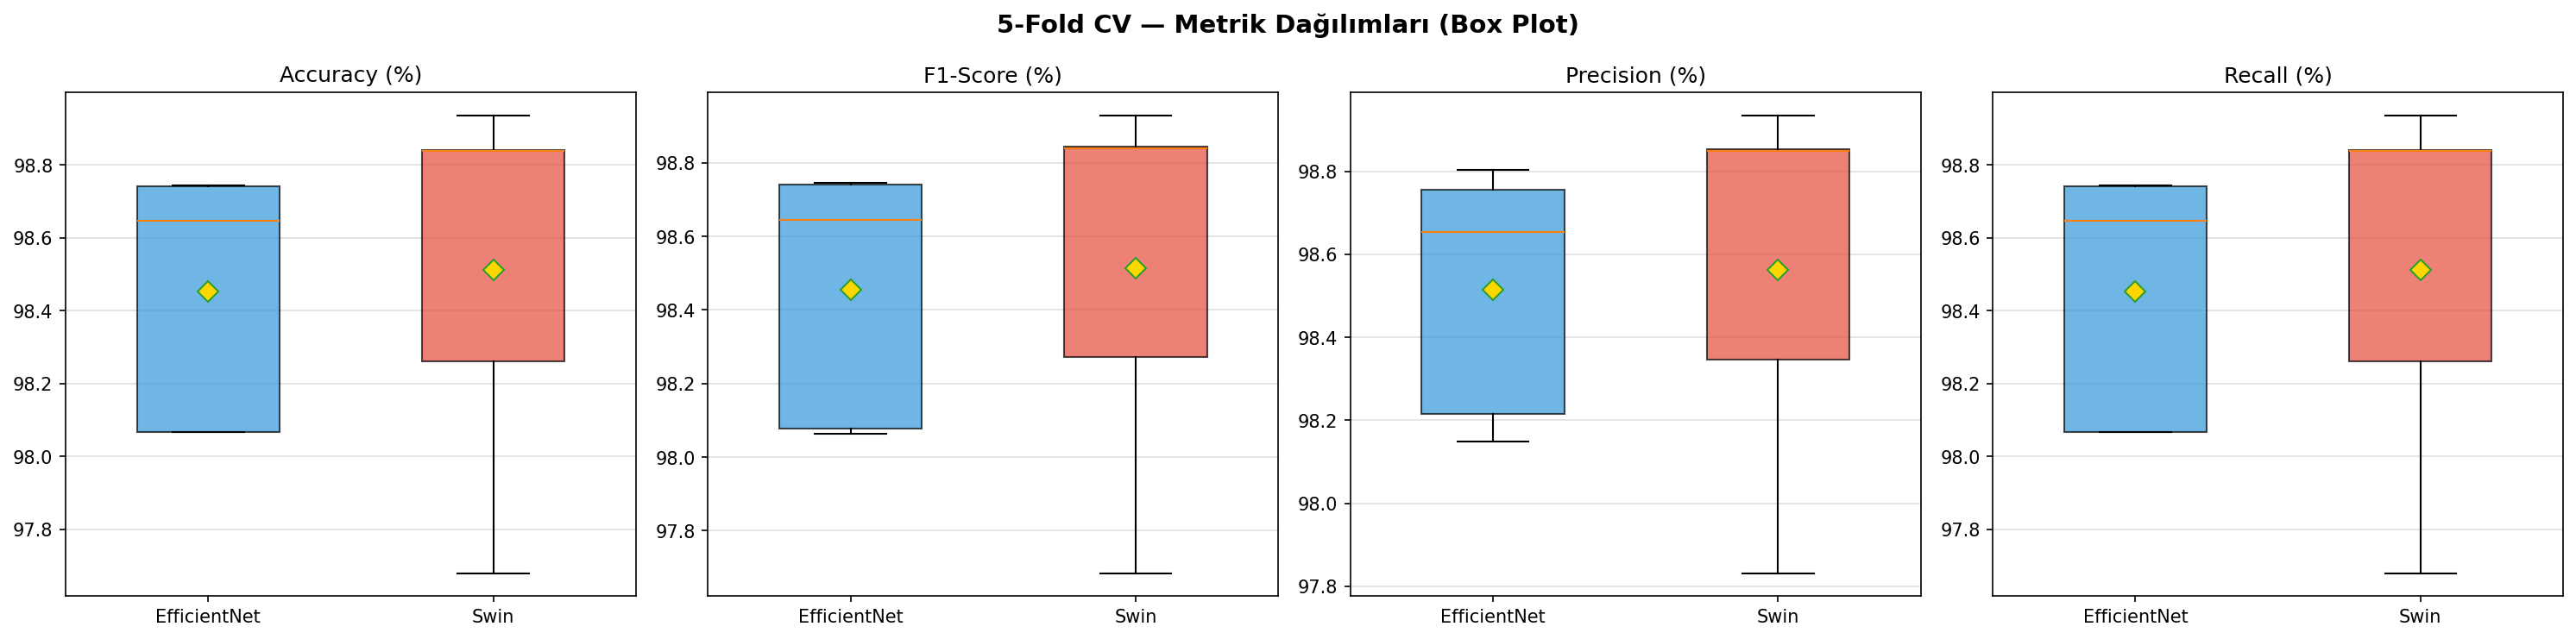
\includegraphics[width=\columnwidth]{fig10_kfold_boxplot.png}
\caption{5-Fold CV metrik dağılımları (Box Plot). Dört temel metrik için EfficientNet ve Swin Transformer'ın kutu grafiği ile karşılaştırılması. Sarı elmas ortalama, turuncu çizgi medyan değeri temsil etmektedir.}
\label{fig:kfold_boxplot}
\end{figure}

Şekil~\ref{fig:kfold_results} ve \ref{fig:kfold_boxplot}'deki görselleştirmeler birlikte değerlendirildiğinde şu çıkarımlar elde edilmektedir: (1)~Her iki model de tüm fold'larda \%97,5'in üzerinde tutarlı performans göstermektedir. (2)~Swin Transformer ortalama olarak küçük bir üstünlük sağlamakla birlikte daha geniş bir dağılıma sahiptir. (3)~EfficientNetV2-S daha düşük standart sapma ile daha kararlı sonuçlar üretmektedir. (4)~Kutu grafiklerinde aykırı değer bulunmaması, her iki modelin de herhangi bir fold'da ciddi performans düşüşü yaşamadığını göstermektedir. Bu sonuçlar, Bölüm~5.2'de tek fold üzerinden raporlanan performansların istatistiksel olarak güvenilir olduğunu teyit etmektedir.

% ════════════════════════════════════════
\section{Tartışma}
% ════════════════════════════════════════

\textbf{Swin Transformer'ın üstünlüğü:} Pencere tabanlı öz-dikkat mekanizması, hastalık belirtilerinin hem yerel (doku, renk) hem de küresel (vücut şekli, uzamsal düzenleme) bağlamda modellenmesine olanak tanımaktadır. Bu özellik, ince görsel farklılıkların kritik olduğu hastalık tespiti görevlerinde belirleyici avantaj sağlamaktadır.

\textbf{Ensemble'ın sınırlı katkısı:} Ensemble modelinin Swin Transformer'ı aşamaması, iki modelin benzer hata örüntüleri sergilediğine işaret etmektedir. Farklı mimari ailelerinden modellerin birleştirilmesi tipik olarak daha belirgin iyileşmeler sağlamakla birlikte bu sonuç veri setinin doğasına özgü sınırlılıklara da işaret etmektedir.

\textbf{Hibrit yaklaşımın değeri:} Hibrit CNN+Gradyan Artırma, uçtan uca modellerle rekabet edememesine karşın yorumlanabilirlik ve hesaplama verimliliği açısından avantaj sunan bir alternatif olarak değerlendirilebilir.

% ════════════════════════════════════════
\section{Sonuç}
% ════════════════════════════════════════

Bu çalışmada, bal arısı hastalıklarının otomatik tespiti için derin öğrenme tabanlı kapsamlı bir karşılaştırmalı analiz sunulmuştur. BeeImage veri setinde Swin Transformer ilk kez uygulanmış ve \%98,74 doğruluk ile mevcut literatür rekorunu (\%98,65) aşmıştır. EfficientNetV2-S + Swin Transformer ensemble modeli F1 skoru bakımından önceki en iyi çalışmaları geride bırakmıştır.

Temel bulgu olarak, Transformer tabanlı mimarilerin küçük ve dengesiz tarımsal görüntü veri setlerinde güçlü bir potansiyele sahip olduğu ortaya konmuştur. Gelecek çalışmalarda daha büyük veri setleri üzerinde doğrulama, gerçek zamanlı izleme sistemlerine entegrasyon ve aktif öğrenme yoluyla etiketleme maliyetinin azaltılması hedeflenmektedir.

% ════════════════════════════════════════
% KAYNAKLAR
% ════════════════════════════════════════

\begin{thebibliography}{13}

\bibitem{uzen2019}
H.~Üzen, İ.~Türkoğlu, and F.~Ata, ``Honey bee diseases and pests diagnosis system using deep learning,'' in \emph{Int.\ Conf.\ Intelligent Systems}, 2019, pp.~47--52.

\bibitem{margapuri2020}
V.~Margapuri, S.~Namburu, and S.~A.~Karre, ``Honey bee colony and varroa mite detection using deep neural networks,'' in \emph{IEEE EIT}, 2020, pp.~548--553.

\bibitem{metlek2021}
S.~Metlek and K.~Kayaalp, ``Classification of honey bee health conditions using deep learning,'' \emph{Computers and Electronics in Agriculture}, vol.~188, p.~106338, 2021.

\bibitem{chawane2022}
M.~Chawane, S.~Viriri, and M.~Gwetu, ``Bee disease identification using DenseNet-121,'' in \emph{ICAICV}, 2022, pp.~212--221.

\bibitem{karthiga2021}
M.~Karthiga, S.~A.~Mary, and J.~Yogapriya, ``Performance analysis of honey bee disease identification using deep learning,'' \emph{J.\ Physics: Conf.\ Series}, vol.~1767, no.~1, p.~012017, 2021.

\bibitem{kaplan2021}
S.~Kaplan~Berkaya, E.~Gunduz~Demir, and S.~Gunal, ``A vision-based bee identification approach using VGG-19,'' \emph{Ecological Informatics}, vol.~65, p.~101425, 2021.

\bibitem{liang2022}
X.~Liang, ``Automated bee disease detection using deep convolutional neural networks,'' \emph{Comp.\ Intel.\ Neuroscience}, vol.~2022, p.~9415538, 2022.

\bibitem{yoo2023}
H.~Yoo, J.~Kim, and S.~Park, ``BeeNet: A specialized deep learning framework for bee disease classification,'' \emph{Computers in Biology and Medicine}, vol.~154, p.~106579, 2023.

\bibitem{kilic2024}
V.~Kılıç and O.~Yaman, ``A color moments-based method for detection of honey bee diseases,'' \emph{Ecological Informatics}, vol.~79, p.~102392, 2024.

\bibitem{yang2018}
J.~Yang, ``BeeImage Dataset: Annotated Honey Bee Images from Video Footage,'' Harvard Dataverse, V1, 2018.

\bibitem{tan2021}
M.~Tan and Q.~V.~Le, ``EfficientNetV2: Smaller models and faster training,'' in \emph{ICML}, 2021, pp.~10096--10106.

\bibitem{liu2021}
Z.~Liu \emph{et~al.}, ``Swin Transformer: Hierarchical vision transformer using shifted windows,'' in \emph{ICCV}, 2021, pp.~10012--10022.

\bibitem{selvaraju2017}
R.~R.~Selvaraju \emph{et~al.}, ``Grad-CAM: Visual explanations from deep networks,'' in \emph{ICCV}, 2017, pp.~618--626.

\end{thebibliography}

\end{document}
